\documentclass[10pt, paper=letter]{scrartcl} % tabellarischer Lebenslauf
\usepackage[american]{babel}
\RequirePackage{makecmds}

\usepackage[utf8]{inputenc}
\usepackage[T1]{fontenc}
\usepackage[letterpaper,left=2cm, right=2cm, top=2.5cm, bottom=2cm]{geometry}

\usepackage{currvita,graphicx,microtype,csquotes,xcolor,doipubmed,charter,fancyhdr,lastpage,soul}

%\usepackage[defaultsans,oldstyle,scale=0.95]{opensans}
\usepackage[default]{FiraSans}
%\renewcommand{\familydefault}{\sfdefault}
\renewcommand{\familydefault}{\rmdefault}

\usepackage[bookmarks,hidelinks]{hyperref}
\usepackage[hyphenbreaks]{breakurl}

\usepackage[shortcuts]{extdash} % hyphenation rules for dashes: - : \-/(no hyphenation: \=/) | -- : \-- (\==) | --- : \--- (\===)  

%\date{April 15, 2019}
%\cvplace{Thunder Bay, ON}

\pagestyle{fancy}
\renewcommand{\headrulewidth}{0pt}
\lhead{\color{gray}\textsf{\MakeUppercase{Curriulum vit\ae}}}
\chead{}
\rhead{\color{gray}\textsf{Tobias Stephan}}
%\rhead{}
%\cfoot{\thepage/11}
\cfoot{\color{gray}\textsf{\thepage\ of \pageref{LastPage}}}

\renewcommand{\thefootnote}{\fnsymbol{footnote}} 

\setkomafont{section}{\Large\scshape\MakeLowercase}
\setkomafont{subsection}{\large}


\begin{document}

\addcontentsline{toc}{chapter}{Curriculum Vitae}

\begin{cv}{\textsf{Dr Tobias Stephan}}
    \medskip
    % \noindent\begin{minipage}{.74\linewidth}%
    %\medskip
    \noindent  Postdoctoral associate\smallskip \\
    Lakehead University\\
    Department of Geology\\
    Thunder Bay, ON, Canada\smallskip \\
    %Earth Sciences, Calgary, AB, T2N 1N4 \smallskip \\
    \noindent Email: \href{mailto:tstephan@lakeheadu.ca}{tstephan@lakeheadu.ca}\\
    Website: \url{https://tobiste.github.io/}\\
    ORCID: \href{https://orcid.org/0000-0002-9290-014X}{0000-0002-9290-014X}
    % \bigskip
    % \end{minipage}%
    % \hfill
    % \begin{minipage}{.24\linewidth}%
    % \raggedleft
    %   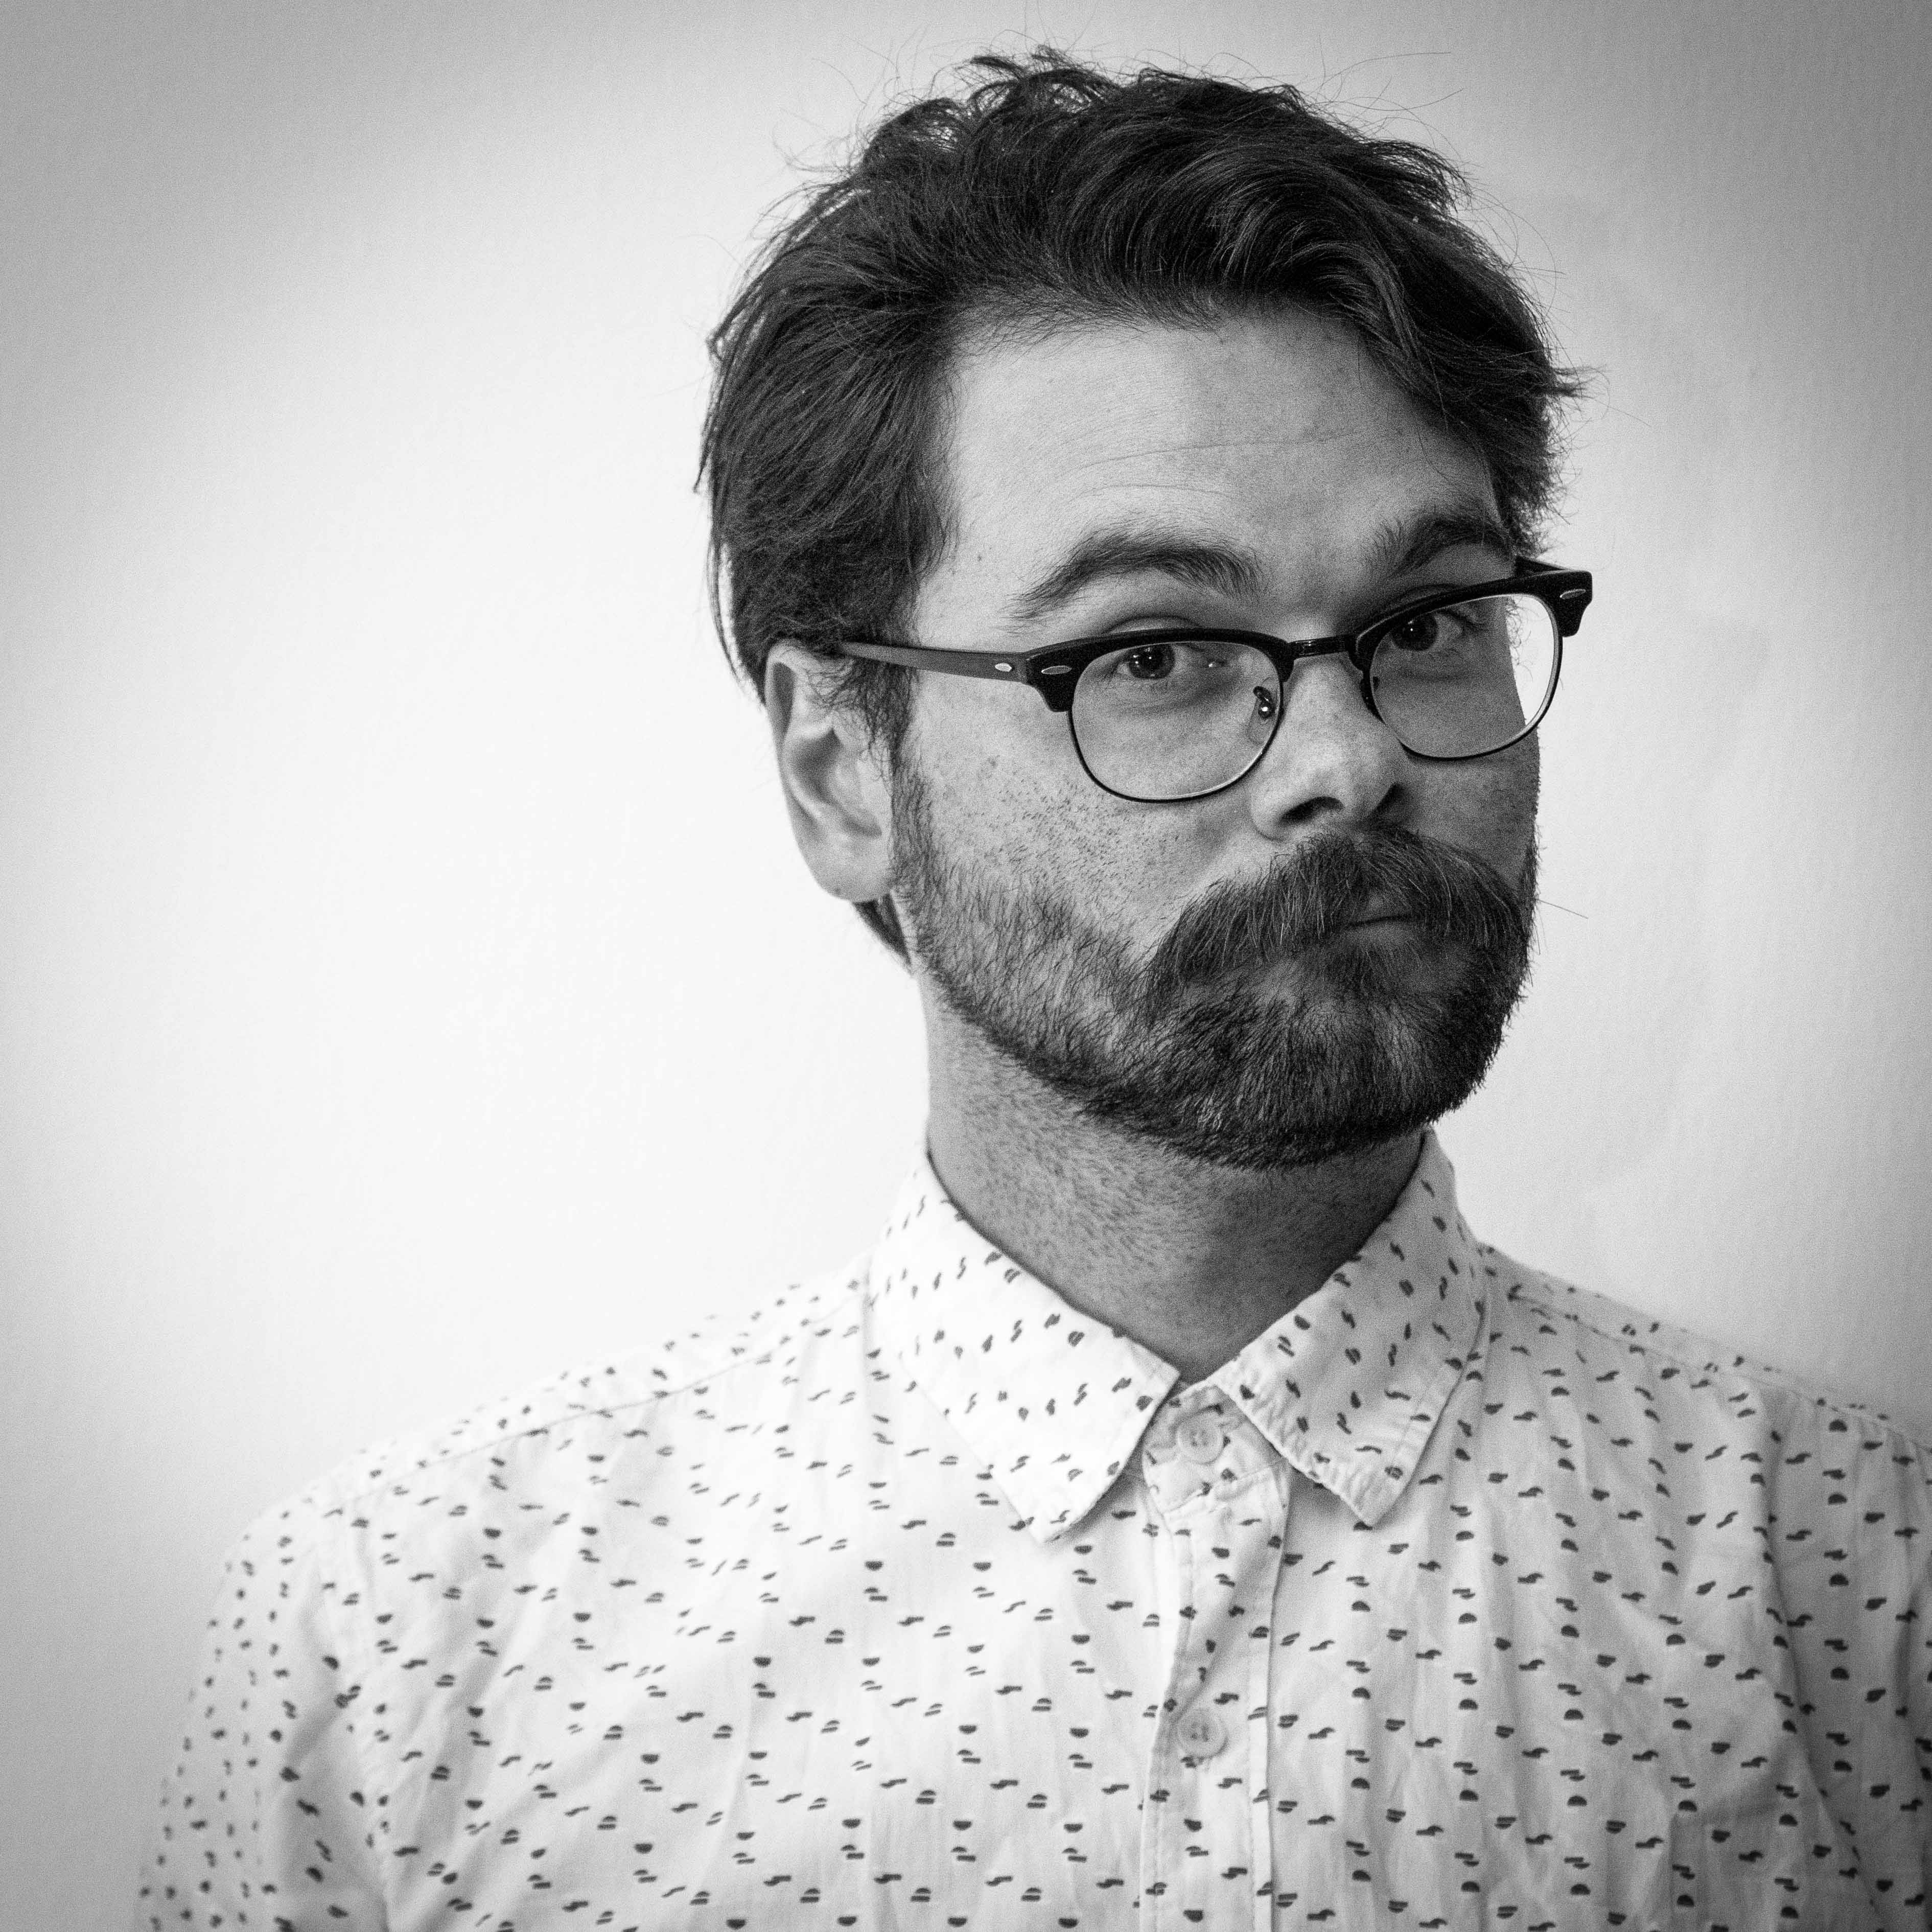
\includegraphics[width = \linewidth]{tobi.jpg}
    % \end{minipage}%

    %\medskip

    % \noindent {\large \textbf{Research interests}}
    % \begin{itemize}\setlength\itemsep{-0.2em}
    %     \item Convergent tectonics
    %     \item Analysis of large-scale patterns of stress and strain fields and their link to tectonic forces
    %     \item Analysis of plate motion
    %     \item Plate tectonic reconstructions
    %     \item Structural analysis of polyphase brittle and ductile deformation
    %     \item Sedimentary provenance analysis
    %     \item Exloring and analysing large geo-datasets using modern statistical tools
    %     \item Paleozoic tectonics of the Variscides
    %     \item Cenozoic tectonics of central Europe and Canadian Cordillera
    % \end{itemize}
    % 
    % 
    % \smallskip

    \section{Education}
    \begin{cvlist}{}
        \item[2019/03] \textbf{Doctor of Philosophy (PhD)} in \enquote{Geology}\\ \textit{Technische Universit\"at Bergakademie Freiberg, Germany}
           
        \item[2013/09] \textbf{Master of Science (MSc)} in \enquote{Geosciences} (major: Tectonics and Geochronology)\\
        \textit{Technische Universit\"at Bergakademie Freiberg, Germany}
           
        \item[2010/09] \textbf{Bachelor of Science (BSc)} in \enquote{Geology and Mineralogy}\\
        \textit{Technische Universit\"at Bergakademie Freiberg, Germany}
     
    \end{cvlist}

    \section{Professional Experience}
    \begin{cvlist}{}
    %\item[since 2025/08]  \textbf{Assistant Professor}\\ \textit{Lakehead University,
    %        Department of Geology, Thunder Bay, ON, Canada}
        \item[since 2023/04] \textbf{Postdoctoral associate}\\ \textit{Lakehead University,
            Department of Geology, Thunder Bay, ON, Canada}
        \item[since 2024/09] \textbf {Lecturer}\\ \textit{Lakehead University, Department of
            Geology, Thunder Bay, ON, Canada}       

        \item[2020/12--2022/11] \textbf{Postdoctoral associate} (DFG Research Fellow)\\
        \textit{University of Calgary, Geo- and Thermochronology Research Group, Department of Geoscience, Calgary, AB, Canada}\
        \item[2020/03--2020/11] \textbf{Postdoctoral associate}\\
        \textit{Friedrich-Alexander-Universit\"at Erlangen-N\"urnberg, Geozentrum Nordbayern, \mbox{Erlangen}, Germany} 
        \item[2019/09--2019/12] \textbf{Research assistant}\\
        \textit{Technische Universit\"at Bergakademie Freiberg, Institute for Computer Sciences, Freiberg, Germany}
        		
        \item[2014/01--2014/06] \textbf{Geologist}\\
        \textit{Beak Consultants GmbH (Germany\,/\,Tanzania)}
        	
      
    \end{cvlist}

    

    %\newpage 
    \section{Publications}
    \subsection{Peer-reviewed articles}
    \setul{1pt}{.4pt}% set underline 1pt below contents
    \begin{cvlist}{}
        %\item[total times cited:] 267\footnote[1]{Web of Science} (362\footnote[2]{Google Scholar})
        % \item[h-index:] 6\footnotemark[1] (7\footnotemark[2])
        %\item[-] \ul{Stephan, T.}  Phillips, N., Tiitto, H., and Hollings, P. \enquote{Going with the flow --- Changes of  Vorticity Controls Gold Enrichment in Archean Shear Zones (Shebandowan Greenstone Belt, Superior Province, Canada)}. submitted to \textit{Structural Geology} in February 2025.
        
        %\item[-] Duschl, F., \ul{Stephan, T.}, K\"ohler, S., Drews, M., Koehn, D., and Stollhofen, H. \enquote{How continents (de-)form: A paleostress chart for Central Europe}. submitted to \textit{Geology} in August 2024.
        \item[15] \ul{Stephan, T.}, and Enkelmann, E. \enquote{All Aligned on the Western Front of North America? Analyzing the Stress Field in the Northern Cordillera}. accepted in \textit{Tectonics} in August 2025.

        \item[14] Padgett, J., Enkelmann, E., Kellett, D., Moynihan, D., and \ul{Stephan, T.} (2025): \enquote{Cenozoic faulting in the Upper Hyland River Valley, Southeastern Yukon: A thermochronological perspective}. \textit{Canadian Journal of Earth Sciences}. \doi{10.1139/cjes-2024-0147}.
        
        \item[13] Schaeben, H., Kroner, U., and \ul{Stephan, T.} (2024): \enquote{Mathematical Fundamentals of Spherical Kinematics of Plate Tectonics in Terms of Quaternions}. \textit{Mathematical Models and Methods in Applied Sciences} 47(6). pp. 4469--4496. \doi{10.1002/mma.9823}

        \item[12] \ul{Stephan, T.}, Enkelmann, E., and Kroner, U. (2023): \enquote{Analyzing the horizontal orientation of the crustal stress adjacent to plate boundaries}. \textit{Scientific Reports} 13:15590. \doi{10.1038/s41598-023-42433-2}.
        %
        \item[11] Járóka, T.,  Pfänder, J.\,A., Seifert, T., Hauff, F., Sperner, B., Staude, S., \ul{Stephan, T.}, and Schulz, B. (2023): \enquote{Age and petrogenesis of Ni-Cu-(PGE) sulfide-bearing gabbroic intrusions in the Lausitz Block, northern Bohemian Massif (Germany/Czech Republic)}. \textit{Lithos} 444--445:107090. \doi{10.1016/j.lithos.2023.107090}
        %
        \item[10] Kroner, U., Romer, R.\,L., and \ul{Stephan, T.} (2023): \enquote{Die Rekonstruktion von relativen Plattenbewegungen aus dem paläozoischen Deformationsmuster der kontinentalen Kruste}. \textit{Zeitschrift der Deutschen Gesellschaft für Geowissenschaften (J. Appl. Reg. Geol.)}. \doi{10.1127/zdgg/2023/0365}
        %
        \item[9] K\"ohler, S., Duschl, F., Fazlikhani, H., Koehn, D., \ul{Stephan, T.}, and Stollhofen, H. (2022): \enquote{Reconstruction of cyclic Mesozoic-Cenozoic stress development in SE Germany using fault-slip and stylolite inversion}. \textit{Geological Magazine} 159 (11--12). pp. 2323--2345.\newline
        \doi{10.1017/S0016756822000656}
        %
        \item[8] Kroner, U., \ul{Stephan, T.}, and Romer, R.\,L. (2022): \enquote{Paleozoic orogenies and relative plate motions at the sutures of the Iapetus-Rheic Ocean}. In Y.\,D. Kuiper, J.\,B. Murphy, R.\,D. Nance, R.\,A. Strachan, and M.\,D. Thompson (Eds.), \textit{New Developments in the Appalachian-Caledonian-Variscan Orogen}. Geological Society of America. \doi{10.1130/2021.2554(01)}
        %
        \item[7] Schaeben, H., Kroner, U., and \ul{Stephan, T.} (2021): \enquote{Euler Poles of Tectonic Plates}. In B.\,S. Daza Sagar, Q. Cheng, J. McKinley, and F. Agterberg (Eds.), \textit{Encyclopedia of Mathematical Geosciences. Encyclopedia of Earth Sciences Series. Springer Nature} Switzerland AG 2021. \doi{10.1007/978-3-030-26050-7\_435-1}
        %
        \item[6] Caracciolo, L., Ravid\`a, D.\,C.\,G., Chew, D., Jan{\ss}en, M., L\"unsdorf, N.\,K., Heins, W.\,A., \ul{Stephan, T.}, and Stollhofen, H. (2021): \enquote{Reconstructing environmental signals across the Permian-Triassic boundary in the SE Germanic Basin: A Quantitative Provenance Analysis (QPA) approach}. \textit{Global and Planetary Change}, 206:103631.  \doi{10.1016/j.gloplacha.2021.103631}
        \item[5] Kroner, U., \ul{Stephan, T.}, Romer, R.\,L., and Roscher, M. (2020): \enquote{Paleozoic plate kinematics during the Pannotia--Pangaea supercontinent cycle}. \textit{Geological Society, London, Special Publications} 503, SP503-2020-15. \doi{10.1144/SP503-2020-15}
        %
        \item[4] \ul{Stephan, T.}, Kroner, U., Romer, R.\,L., and R\"osel, D. (2019): \enquote{From a bipartite Gondwana shelf to the arcuate Variscan belt: The Early Paleozoic evolution of northern Peri-Gondwana}. \textit{Earth-Science Reviews} 192, pp. 491--512. \doi{10.1016/j.earscirev.2019.03.012}
        %
        \item[3] Heinicke, J., \ul{Stephan, T.}, Alexandrakis, C., Buske, S., and Gaupp, R. (2019): \enquote{Alteration as possible cause for transition from brittle failure to aseismic slip: the case of the NW-Bohemia\,/\, Vogtland earthquake swarm region}. \textit{Journal of Geodynamics} 124, pp. 79--92. \doi{10.1016/j.jog.2019.01.010}
        %
        \item[2] \ul{Stephan, T.}, Kroner, U., and Romer, R.\,L. (2018): \enquote{The pre-orogenic detrital zircon record of the Peri-Gondwanan crust}. \textit{Geological Magazine} 156\,(2), pp. 281--307.\newline
        \doi{10.1017/s0016756818000031}.
        %
        \item[1] \ul{Stephan, T.}, Kroner, U., Hahn, T., Hallas, P., and Heuse, T. (2016): \enquote{Fold\,/\,cleavage relationships as indicator for late Variscan sinistral transpression at the Rheno\-/Hercynian\--Saxo\-/Thuringian boundary zone, Central European Variscides}. \textit{Tectonophysics} 681, pp. 250--262. \doi{10.1016/j.tecto.2016.03.005}
    \end{cvlist}

    \subsection{Other academic articles}
    \begin{cvlist}{}
        \item[Book] Legler, C., Barth, A., Knobloch, A., Mruma, A.\,H., Myumbilwa Y.,
        Magigita, M., Msechu, M., Ngole, T., Stanek, K.\,P., Boniface, N., Kagya, M.,
        Manya, S., Berndt, T., Stahl, M., Gebremichael, M., Dickmayer, E., Repper, C.,
        Falk, D., and Stephan, T. (2015): \enquote{Explanatory Notes for the
            Minerogenic Map of Tanzania 1:1,5 M.}, \textit{Geological Survey of Tanzania}.
        ISBN: 978-9987-477-94-4
    \end{cvlist}

    \section{Software developments}
    \begin{cvlist}{}
        \item[\texttt{tectonicr}] Free and open-source R package for modeling and analyzing the direction of the maximum horizontal stress using relative plate motion (\doi{10.32614/CRAN.package.tectonicr}).\\
        Package website: \url{https://tobiste.github.io/tectonicr/}
        \item[\texttt{structr}] Free and open-source R package for analyzing and visualizing orientation data for structural geology.
        \url{https://github.com/tobiste/structr}
        \item[\texttt{geoprofiler}] Creates Swath profiles and Distance vs X plots by measuring the accurate distances parallel and perpendicular to user-defined lines.
        \url{https://tobiste.github.io/geoprofiler/}
        \item[\texttt{ptrotR}] Free and open-source R package for plate motion reconstruction.\\
        \url{https://github.com/tobiste/ptrotR}
        \item[\texttt{laftr}] Free and open-source R package to calculate the ages from LA-ICP-MS based fission track dating using the zeta approach.
        \url{https://github.com/tobiste/laftr}
        \item[\texttt{euler}] Free and open-source R package for describing plate motion in terms of quaternions.\newline
        \url{https://github.com/tobiste/euler}
        \item[\texttt{euler.reco}] Free and open-source R package. Provides algorithms to find and evaluate the Euler pole solution describing the orientation of geological structures.\\
        \url{https://github.com/tobiste/euler.reco}
    \end{cvlist}

    %\newpage
    \section{Funding, Grants, and Awards}
    \begin{cvlist}{}
        \item[Grants] 2020--2022
        \href{https://gepris.dfg.de/gepris/projekt/439621066?language=en}{DFG Research
            Fellowship} (85\,000\texteuro) --- \textit{German Research Foundation (DFG)}
        \item[] 2016 Travel grant (750\texteuro) --- \textit{Centre of Advanced Study and Research Freiberg}
        \item 2013 Travel grant (500\texteuro) --- \textit{TU Bergakademie Freiberg Association of Friends}
        \item 2009 IAESTE Internship stipend --- \textit{International Association for the Exchange of Students for Technical Experience
            (IAESTE)}
        \item[Awards] Poster award at \textit{CETEG2015}, Kada\v{n}, Czech Republic, 2014
    \end{cvlist}

    \section{Professional Services and Memberships}
    \begin{cvlist}{}
        \item[Memberships] The Geological Association of Canada (GAC), Canadian Tectonics
        Group (CTG)%, American Geophysical Union (AGU), European Geological Union (EGU), German Geological Union and Society (DGGV)
        \item[Reviewer for journals] Geology, Gondwana Research, Terra Nova, Geological
        Society of America, Scientific Reports, Proceedings of the Geologists'
        Association, Basin Research, Lithosphere, Discover Geoscience, Tectonics
        \item[Reviewer for grant proposals] National Science Center, Poland
        \item[Committee board member] Jack Henderson Best PhD Thesis Award from the Canadian
        Tectonics Group of the GAC (since 2023)
        \item[Session Chair] \textit{GAC-MAC-PEG 2024} (Brandon, MN, Canada): \enquote{It’s
            our fault! Geological and geophysical insights into fault and shear zone
            processes}
    \end{cvlist}

\end{cv}
\end{document}
